% Preamble.
\documentclass[12pt]{article}
\usepackage[utf8x]{inputenc}
\usepackage{color,
            hyperref,
            fancyhdr,
            xcolor,
            enumitem,
            amssymb,  % More math commands.
            amsmath,
            tikz,
            changepage,
            algorithmic,
            }
\usepackage[textwidth=16.625cm]{geometry}
\usepackage{graphicx}
\usepackage[ruled]{algorithm2e}
\usepackage{tikz-qtree}

% Commands.
\renewcommand{\headrulewidth}{0.0pt}
\newcommand{\ts}{\textsuperscript}
\newcommand{\ul}{\underline}
\newcommand\tab[1][1cm]{\hspace*{#1}}
\def\checkmark{\tikz\fill[scale=0.4](0,.35) -- (.25,0) -- (1,.7) -- (.25,.15) -- cycle;} % Checkmark
\def\code#1{\texttt{#1}}  % Write code.
% Email Command.
\providecommand*\emaillink[1]{\nolinkurl{#1}}
\providecommand*\email[1]{\href{mailto:#1}{\emaillink{#1}}}

% Style.
\pagestyle{fancy}
\chead{CSC 460 -- Database Design\\ Fall 2021 (McCann)}
\cfoot{\thepage}
\urlstyle{same}
% Link Style.
\hypersetup{colorlinks,
            urlcolor=[RGB]{6, 69, 173},
            linkbordercolor=[RGB]{6, 69, 173},
            pdfborderstyle={/S/U/W 1}
            }
% Set wider margins to give more text per page.
\setlength{\topmargin}{-0.50in}     % in == inches (others:  cm, mm, pt, ...)
\setlength{\textheight}{9.25in}     % what's left-over is the bottom margin
\setlength{\textwidth}{6.625in}
\setlength{\oddsidemargin}{0.0in}   % right-side pages in a magazine
\setlength{\evensidemargin}{0.0in}  % left-side

\setlength{\parindent}{0.0cm}	    % don't indent first lines of paragraphs
\setlength{\parskip}{0.4cm}         % distance between paragraphs

% Body.
\begin{document}

% Header Stuff.
\begin{center}
{\Large \textbf{Program \#4: Database Design and Implementation}}\\
\textit{Due Date: December 6\ts{th}, 2021, \underline{at the beginning of class}}

\ul{Danny Ryngler -- \code{\email{dryngler@email.arizona.edu}}}
\ul{James O'Connell -- \code{\email{oconnellj2@email.arizona.edu}}}
\end{center}

\section*{1  Conceptual Database Design}
\fbox{\begin{minipage}{6.72in}
	\tikzset{every picture/.style={line width=0.75pt}} %set default line width to 0.75pt        

	\begin{tikzpicture}[x=0.75pt,y=0.75pt,yscale=-1,xscale=1]
	%uncomment if require: \path (0,653); %set diagram left start at 0, and has height of 653

	%Straight Lines [id:da43139336388917227] 
	\draw    (20,286) -- (98,286) ;
	%Straight Lines [id:da4834284295403961] 
	\draw    (282,270) -- (378,270) ;
	%Straight Lines [id:da10761222840211937] 
	\draw    (304,26) -- (357,26) ;
	%Straight Lines [id:da7255206002748934] 
	\draw    (553,274) -- (636.88,273.85) ;
	%Straight Lines [id:da6995347636449339] 
	\draw    (537.82,26.88) -- (649,27) ;
	%Straight Lines [id:da9523894723443324] 
	\draw    (33,484) -- (80.88,483.85) ;
	%Straight Lines [id:da22513051522654337] 
	\draw    (289,469) -- (366.88,468.85) ;
	%Straight Lines [id:da07760638923345364] 
	\draw    (549,506) -- (640,506) ;
	%Straight Lines [id:da5775438824489482] 
	\draw    (98,304) -- (282,304.8) ;
	%Straight Lines [id:da4262009384989398] 
	\draw    (378,305) -- (553,305.8) ;
	%Straight Lines [id:da5168381269792842] 
	\draw    (367,508.2) -- (549,509) ;
	%Straight Lines [id:da8759115752898501] 
	\draw    (81,507) -- (289,507.8) ;
	%Straight Lines [id:da831087986862331] 
	\draw    (594,476.5) -- (594,360.5) ;
	%Straight Lines [id:da19235984180779042] 
	\draw    (330,240) -- (330,70) ;
	%Straight Lines [id:da5249140419115729] 
	\draw    (593,251) -- (593,135) ;

	% Text Node
	\draw    (20,261) -- (98,261) -- (98,349) -- (20,349) -- cycle  ;
	\draw (23,265) node [anchor=north west][inner sep=0.75pt]   [align=left] {\begin{minipage}[lt]{50.37pt}\setlength\topsep{0pt}
	\begin{center}
	Customer\\\underline{cust\_id}\\first\_name\\last\_name
	\end{center}

	\end{minipage}};
	% Text Node
	\draw    (282,240) -- (378,240) -- (378,370) -- (282,370) -- cycle  ;
	\draw (285,244) node [anchor=north west][inner sep=0.75pt]   [align=left] {\begin{minipage}[lt]{62.85pt}\setlength\topsep{0pt}
	\begin{center}
	Appointment \\\underline{app\_id}\\cust\_id\\service\_id\\app\_date\\success
	\end{center}

	\end{minipage}};
	% Text Node
	\draw    (304,3) -- (357,3) -- (357,70) -- (304,70) -- cycle  ;
	\draw (307,7) node [anchor=north west][inner sep=0.75pt]   [align=left] {\begin{minipage}[lt]{33.38pt}\setlength\topsep{0pt}
	\begin{center}
	Xact\\\underline{app\_id}\\fee
	\end{center}

	\end{minipage}};
	% Text Node
	\draw    (553,251) -- (637,251) -- (637,360) -- (553,360) -- cycle  ;
	\draw (556,255) node [anchor=north west][inner sep=0.75pt]   [align=left] {\begin{minipage}[lt]{54.34pt}\setlength\topsep{0pt}
	\begin{center}
	Service\\\underline{service\_id}\\name\\fee\\years\_valid
	\end{center}

	\end{minipage}};
	% Text Node
	\draw    (538,5) -- (649,5) -- (649,135) -- (538,135) -- cycle  ;
	\draw (541,9) node [anchor=north west][inner sep=0.75pt]   [align=left] {\begin{minipage}[lt]{72.52pt}\setlength\topsep{0pt}
	\begin{center}
	Document\\\underline{docid}\\service\_id\\cust\_id\\issue\_date\\expiration\_date
	\end{center}

	\end{minipage}};
	% Text Node
	\draw    (33,462) -- (81,462) -- (81,550) -- (33,550) -- cycle  ;
	\draw (36,466) node [anchor=north west][inner sep=0.75pt]   [align=left] {\begin{minipage}[lt]{29.94pt}\setlength\topsep{0pt}
	\begin{center}
	Job\\\underline{jid}\\title\\salary
	\end{center}

	\end{minipage}};
	% Text Node
	\draw    (289,444) -- (367,444) -- (367,574) -- (289,574) -- cycle  ;
	\draw (292,448) node [anchor=north west][inner sep=0.75pt]   [align=left] {\begin{minipage}[lt]{50.37pt}\setlength\topsep{0pt}
	\begin{center}
	Employee\\\underline{eid}\\jid\\did\\first\_name\\last\_name
	\end{center}

	\end{minipage}};
	% Text Node
	\draw    (549,477) -- (640,477) -- (640,544) -- (549,544) -- cycle  ;
	\draw (552,481) node [anchor=north west][inner sep=0.75pt]   [align=left] {\begin{minipage}[lt]{58.88pt}\setlength\topsep{0pt}
	\begin{center}
	Department \\\underline{did}\\name
	\end{center}

	\end{minipage}};
	% Text Node
	\draw (164,285) node [anchor=north west][inner sep=0.75pt]   [align=left] {custApp};
	% Text Node
	\draw (307,143) node [anchor=north west][inner sep=0.75pt]   [align=left] {log};
	% Text Node
	\draw (441,287) node [anchor=north west][inner sep=0.75pt]   [align=left] {appService};
	% Text Node
	\draw (511,408) node [anchor=north west][inner sep=0.75pt]   [align=left] {deptService};
	% Text Node
	\draw (425,490) node [anchor=north west][inner sep=0.75pt]   [align=left] {empDept};
	% Text Node
	\draw (159,488) node [anchor=north west][inner sep=0.75pt]   [align=left] {empJob};
	% Text Node
	\draw (100,307) node [anchor=north west][inner sep=0.75pt]   [align=left] {$\displaystyle 0...*$};
	% Text Node
	\draw (332,73) node [anchor=north west][inner sep=0.75pt]   [align=left] {$\displaystyle 0...*$};
	% Text Node
	\draw (519,308) node [anchor=north west][inner sep=0.75pt]   [align=left] {$\displaystyle 0...*$};
	% Text Node
	\draw (515,511) node [anchor=north west][inner sep=0.75pt]   [align=left] {$\displaystyle 0...*$};
	% Text Node
	\draw (331,219) node [anchor=north west][inner sep=0.75pt]   [align=left] {$\displaystyle 1...1$};
	% Text Node
	\draw (256,510) node [anchor=north west][inner sep=0.75pt]   [align=left] {$\displaystyle 1...1$};
	% Text Node
	\draw (83,510) node [anchor=north west][inner sep=0.75pt]   [align=left] {$\displaystyle 1...1$};
	% Text Node
	\draw (595,457) node [anchor=north west][inner sep=0.75pt]   [align=left] {$\displaystyle 1...1$};
	% Text Node
	\draw (596,363.5) node [anchor=north west][inner sep=0.75pt]   [align=left] {$\displaystyle 1...4$};
	% Text Node
	\draw (380,308) node [anchor=north west][inner sep=0.75pt]   [align=left] {$\displaystyle 1...*$};
	% Text Node
	\draw (248,307) node [anchor=north west][inner sep=0.75pt]   [align=left] {$\displaystyle 1...*$};
	% Text Node
	\draw (369,511.2) node [anchor=north west][inner sep=0.75pt]   [align=left] {$\displaystyle 0...1$};
	% Text Node
	\draw (516,181) node [anchor=north west][inner sep=0.75pt]   [align=left] {serviceDoc};
	% Text Node
	\draw (595,137) node [anchor=north west][inner sep=0.75pt]   [align=left] {$\displaystyle 1...*$};
	% Text Node
	\draw (594,230) node [anchor=north west][inner sep=0.75pt]   [align=left] {$\displaystyle 1...*$};
	\end{tikzpicture}
\end{minipage}}

\newpage
\section*{2 Logical database design}

\begin{center}
\begin{minipage}{0.5\linewidth}
Customer
\begin{tabular}[l]{|c|c|c|}
	\hline
	\ul{cust\_id} &first\_name &last\_name\\
	\hline
\end{tabular}\\

Appointment
\begin{tabular}[l]{|c|c|c|c|c|}
	\hline
	\ul{app\_id} &cust\_id &service\_id &app\_date &success\\
	\hline
\end{tabular}\\

Xact
\begin{tabular}[l]{|c|c|c|}
	\hline
	\ul{xact\_id} &app\_id &fee\\
	\hline
\end{tabular}\\

Service
\begin{tabular}[l]{|c|c|c|c|}
	\hline
	\ul{service\_id} &name &fee &years\_valid\\
	\hline
\end{tabular}\\

Document
\begin{tabular}[l]{|c|c|c|c|c|}
	\hline
	\ul{docid} &service\_id &cust\_id &issue\_date &expiration\_date\\
	\hline
\end{tabular}\\

Job
\begin{tabular}[l]{|c|c|c|}
	\hline
	\ul{jid} &title &salary\\
	\hline
\end{tabular}\\

Employee
\begin{tabular}[l]{|c|c|c|c|c|}
	\hline
	\ul{eid} &jid &did &first\_name &last\_name\\
	\hline
\end{tabular}\\

Department
\begin{tabular}[l]{|c|c|}
	\hline
	\ul{did} &name\\
	\hline
\end{tabular}

\end{minipage}
\end{center}

\newpage
\section*{3 Normalization analysis}
\ul{Customer}:\\
cust\_id$\rightarrow$first\_name\\
cust\_id$\rightarrow$last\_name\\
1NF: Becasue its attributes are not set-valued.\\
2NF: Every non-prime attribute is fully functionally dependent upon every CK.\\
3NF + BCNF: In both FDs \ul{cust\_id} is a super key of the relation.

\ul{Appointment}:\\
app\_id$\rightarrow$cust\_id\\
app\_id$\rightarrow$service\_id\\
app\_id$\rightarrow$app\_app\_date\\
app\_id$\rightarrow$success\\
1NF: Becasue its attributes are not set-valued.\\
2NF: Every non-prime attribute is fully functionally dependent upon every CK.\\
3NF + BCNF: In both FDs \ul{app\_id} is a super key of the relation.

\ul{Xact}:\\
xact\_id$\rightarrow$app\_id\\
xact\_id$\rightarrow$fee\\
1NF: Becasue its attributes are not set-valued.\\
2NF: Every non-prime attribute is fully functionally dependent upon every CK.\\
3NF + BCNF: In both FDs \ul{xact\_id} is a super key of the relation.

\ul{Service}:\\
service\_id$\rightarrow$name\\
service\_id$\rightarrow$fee\\
service\_id$\rightarrow$years\_valid\\
1NF: Becasue its attributes are not set-valued.\\
2NF: Every non-prime attribute is fully functionally dependent upon every CK.\\
3NF + BCNF: In both FDs \ul{service\_id} is a super key of the relation.

\ul{Document}:\\
doc\_id$\rightarrow$service\_id\\
doc\_id$\rightarrow$cust\_id\\
doc\_id$\rightarrow$expiration\_date\\
1NF: Becasue its attributes are not set-valued.\\
2NF: Every non-prime attribute is fully functionally dependent upon every CK.\\
3NF + BCNF: In both FDs \ul{doc\_id} is a super key of the relation.

\newpage
\ul{Job}:\\
jid$\rightarrow$title\\
jid$\rightarrow$salary\\
1NF: Becasue its attributes are not set-valued.\\
2NF: Every non-prime attribute is fully functionally dependent upon every CK.\\
3NF + BCNF: In both FDs \ul{jid} is a super key of the relation.

\ul{Employee}:\\
eid$\rightarrow$jid\\
eid$\rightarrow$did\\
eid$\rightarrow$first\_name\\
eid$\rightarrow$last\_name\\
1NF: Becasue its attributes are not set-valued.\\
2NF: Every non-prime attribute is fully functionally dependent upon every CK.\\
3NF + BCNF: In both FDs \ul{eid} is a super key of the relation.

\ul{Department}:\\
did$\rightarrow$name\\
1NF: Becasue its attributes are not set-valued.\\
2NF: Every non-prime attribute is fully functionally dependent upon every CK.\\
3NF + BCNF: In both FDs \ul{did} is a super key of the relation.

\newpage
\section*{4 Query description}

\begin{center}
	\begin{minipage}{0.5\linewidth}
	\code{SELECT salary\\
	FROM Job, Employee\\
	WHERE Job.jid $=$ Employee.jid\\
	AND Employee.first\_name $=$ `\%s'\\
	AND Employee.last\_name $=$ `\%s'}
	\end{minipage}
\end{center}

\tab Our self--designed query answers the question: ``What is the salary of a given Employee''. Given the first and last name from the user and by preforming a join on the Employee and Job relations, we are able to determine the answer to this question. The utility of the query allows users to get insight into the people that work at the DMV.
\end{document}